\documentclass[12pt,fleqn]{article}\usepackage{../../common}
\begin{document}
Paralel Matris Çarpımı, Ax, QR ve SVD

[5] adlı yazı tek makinalı ortamda matris çarpımının nasıl yapılacağını, ve
nasıl görülecebileğini anlattı. Satır bakış açısı, kolon bakış açısı
işlendi. Parallel (Hadoop), eşle/indirge ortamında matris çarpımını nasıl
yaparız?  Mesela $A^TA$'yi ele alalım. Bu çarpım oldukça önemli çünkü başka
sonuçlar için de kullanılabiliyor. Mesela $A$ üzerinde $QR$ ayrıştırması
yapmak isterseniz (bkz. Lineer Cebir ders notlarımız) bu çarpım
kullanılabiliyor.

Nasıl? QR ayrıştırması kolonların hepsi bilindiği gibi birbirine dik
(orthogonal) birim vektörler olan bir $Q$ matrisi ve üst üçgensel (upper
triangular) bir $R$ matrisi oluşturur. Ayrıştırmanın $A^TA$ ile bağlantısı
nedir? Eğer $A$ yerine onun ayrıştırmasını $QR$ koyarsak,

$$
C = A^TA = (QR)^T (QR) = R^T Q^T QR
$$

Tum $Q$ vektorleri birbirine dik, ve birim vektorler ise, $Q^T Q$
birim matrisi $I$ olur. O zaman

$$
C = R^T Q^T QR = R^T R
$$

Yani

$$
C = R^TR
$$

Peki $A^TA$ hesaplayıp (böylece $R^TR$'yi elde edince) onun içinden $R$'yi nasıl
çekip çıkartırız? Şimdi Cholesky ayrıştırması kullanmanın zamanı. Cholesky
ayrıştırması (herhangi bir simetrik pozitif kesin $C$ matrisi üzerinde)

$$C = LL^T$$

olarak bilinir, yani bir matris alt üçgensel (lower triangular -ki L harfi
oradan geliyor-) $L$ matrisine ve onun devriği olan üst üçgensel $L^T$'nin
çarpımına ayrıştırılır. Elimizde $R^TR$ var, ve ona benzer $LL^T$ var, $R$
bilindiği gibi üst üçgensel, $L$ alt üçgensel, $L^T$ ve $R$ birbirine eşit demek
ki. Yani $A^TA$ üzerinde sayısal hesap kütüphenimzin Cholesky çağrısı kullanmak
bize $QR$'in $R$'sini verir.

Şu anda akla şu soru gelebilir: madem kütüphane çağrısı yaptık, niye $A$
üzerinde kütüphenimizin $QR$ çağrısını kullanmıyoruz?

Cevap Büyük Veri argümanında saklı. Bu ortamda uğraşılan verilerde $A$ matrisi
$m \times n$ boyutlarındadır, ve $m$ milyonlar, hatta milyarlarca satır
olabilir. Şimdilik $m >> n$ olduğunu farzedelim, yani $m$, $n$'den "çok, çok
büyük", yani "boyut kolonlarının", ki $n$, sayısı binler ya da onbinlerde. Bu
gayet tipik bir senaryo aslında, ölçüm noktaları (boyutlar) var, ama çok fazla
değil, diğer yandan o ölçümler için milyonlarca veri noktası toplanmış. Tipik
bir aşırı belirtilmiş (överdetermined) sistem - ki en az kareler (least squares)
gibi yaklaşımların temel aldığı sistemler bunlardır, eldeki denklem sayısından
daha fazla ölçüm noktası vardır. Bu arada en az karelerden bahsettik, $QR$'in
kullanıldığı alanlardan biri en az karelerin çözümüdür.

Argümana devam ediyoruz, kütüphane \verb!qr! çağrısını $A$ üzerinde yaparsak, $m
\times n$ gibi devasa bir matris üzerinde işlem yapmak gerekir. Ama $A^TA$
üzerinde işlem (Cholesky) yaparsak, ki bu çarpımın boyutu $n \times m \cdot m
\times n = n \times n$, yani çok daha ufak bir matristir. $A^TA$'in işlem bedeli
çok ufak, birazdan anlatacağımız yöntem sayesinde bu bedel $O(m)$.

Paralel $A^TA$

Paralel çarpıma gelelim. Öncelikle elimizdeki becerilere (çapabilities)
bakalım. Hadoop ortamı bize aşırı büyük bir dosyayı otomatik olarak makinalara
bölerek bir hesap yapılması gerektiğinde o hesabın her makinadaki veri parçası
üzerinde yaptırılabilmesini sağlıyor.

$A^TA$ örneğinde eldeki veri $A$, ve "çok olan" $A$'nin satırları, yani $m
\times n$ boyutlarında matris var ve $m$ devasa boyutlarda (olabilir). Bir $A$
dosyası tipik olarak şöyle gözükecek:

\begin{minted}[fontsize=\footnotesize]{python}
!head -5 A_matrix
\end{minted}

\begin{verbatim}
3 4 5 6
3 4 5 2
3 6 7 8
2 2 2 2
9 9 3 3
\end{verbatim}

Eşle/indirgeye gelelim: Eğer çarpıma satır bakışını hatırlarsak,

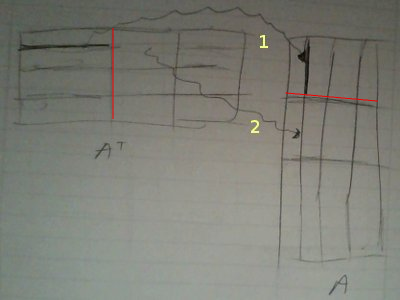
\includegraphics[height=6cm]{AtA.png}

Bu bakışa göre soldaki matriste satır boyunca giderken, sağdakinde ona tekabül
eden kolon boyunca gidiyoruz, ve birbirine eşlene her ögeyi çarpıyoruz, ve
çarpımları topluyoruz.

Şimdi bu matrisin Hadoop'ta parça parça bize geldiğini düşünürsek (ki üstte
hayali bir ilk parçayı kırmızı çizgi ile belirttik), bu parça içinde mesela ilk
satırı kendisi ile çarparken (1'inci ok) aynı blok içindeyiz. Bu önemli bir
nokta, çarparken bloklar arası geçiş yok.

Tabii ki nihai çarpımdaki (1,1) hesabı için $A^T$'deki birinci satırın {\em
  tamamen} $A$'daki birinci kolonla nokta çarpımının bitirilmiş olması gerekir,
ama şimdi düşünelim, başka bir makinaya ikinci parça verilmiş ise, makinada o
birinci satırın geri kalanı çarpılıp toplanacaktır (2. ok), ve eğer tüm
parçalar, tüm makinalarda bu şekilde işlenirse, (1,1) hesabı için o
makinalardaki o tüm çarpımları alıp nihai bir noktada toplamak bize (1,1) için
nihai sonucu verecektir. Bu tipik bir eşle/indirge hesabı olabilir, eşle
safhasında eldeki parça $A_p$ üzerinde $A_p^T A_p$ yapılır, indirge safhasında
bu parçalar toplanır.

Eşleme safhasından yayınlanacak (emit) anahtar ve değerler, bizce, $A_p^T A_p$
içindeki her satırın satır no'su ve satır değeri olmalı. Niye? (Aynı sabit bir
anahtar değeriyle beraber $A_p^T A_p$'in tamamını da yayınlayabilirdik).

Hatırlayalım, nihai çarpım $n \times n$ boyutunda, her parça $p$ olsa bile, $n
\times p \cdot p \times n$ yine bize $n \times n$ veriyor. Yani her makina $n
\times n$ boyutunda bir çarpım sonucunu üretiyor. Evet $n$ nispeten küçük bir
sayı, fakat yine de onbinlerde olsa bile $10,000 \times 10,000$ mesela, büyük
bir sayı. Eğer tüm toplamı tek bir indirgeyici makinaya yaptırırsak, pek çok $n
\times n$ boyutunda matrisin toplamı bu makinayı kaşar. O sebeple indirgeme
sonrası matrisleri değil, o matrislerin her $n$ satırını satır no'su ile
yayınlıyoruz, böylece aynı satırlar aynı indirgeyiciye gidip orada
toplanıyorlar, ama birçok indirgeyici var yani toplama işlemi paralel hale
gelmiş oluyor. Tabii indirgeme sonrası o sonuçlar yayınlanıyor, ve satır no'ya
göre doğal olarak sıralanmış halde nihai sonuç çıkıyor.  Ama toplama işlemi
paralel. Kod alttaki gibi

\inputminted[fontsize=\footnotesize]{python}{AtA.py}

Fonksiyon \verb!mapper_final! MRJob kurallarına göre bir makinadaki tüm eşleme
bittikten sonra çağırılır, biz bu çengeli (hook), "artık parçaları çarpıp
yayınlamak için" kullandık, her parça $p$ büyüklüğünde, ama $m / p$ tam sayı
olmayabilir, yani işlem sonunda bazı artık veriler kalmış olabilir, onları
\verb!mapper_final!  içinde çarpıyoruz.

Bu arada kodun kendi içinde de bir "parçalama", "biriktirme ve işleme" yaptığına
dikkat, yani 20,000 satır olabilir, iki tane eşleyici var ise her eşleyici bu
verinin 10,000 satırını işler, ama ayrıca işleyiciler daha ufak ufak (üstte 4)
parçalarla çarpım yapıyor.

\begin{minted}[fontsize=\footnotesize]{python}
!python AtA.py A_matrix
\end{minted}

\begin{verbatim}
using configs in /home/burak/.mrjob.conf
creating tmp directory /tmp/AtA.burak.20131202.225802.256844
writing to /tmp/AtA.burak.20131202.225802.256844/step-0-mapper_part-00000
Counters from step 1:
  (no counters found)
writing to /tmp/AtA.burak.20131202.225802.256844/step-0-mapper-sorted
> sort /tmp/AtA.burak.20131202.225802.256844/step-0-mapper_part-00000
writing to /tmp/AtA.burak.20131202.225802.256844/step-0-reducer_part-00000
Counters from step 1:
  (no counters found)
Moving /tmp/AtA.burak.20131202.225802.256844/step-0-reducer_part-00000 -> /tmp/AtA.burak.20131202.225802.256844/output/part-00000
Streaming final output from /tmp/AtA.burak.20131202.225802.256844/output
0	"[ 420.  463.  264.  265.]"
1	"[ 463.  538.  351.  358.]"
2	"[ 264.  351.  316.  321.]"
3	"[ 265.  358.  321.  350.]"
removing tmp directory /tmp/AtA.burak.20131202.225802.256844
\end{verbatim}

Karşılaştırmak için aynı işlemi tek bir script içinde yapalım, 

\begin{minted}[fontsize=\footnotesize]{python}
A = np.loadtxt('A_matrix')
print np.dot(A.T,A)
\end{minted}

\begin{verbatim}
[[ 420.  463.  264.  265.]
 [ 463.  538.  351.  358.]
 [ 264.  351.  316.  321.]
 [ 265.  358.  321.  350.]]
\end{verbatim}

Tıpatıp aynı. 

Şimdi bu sonuç üzerinde Cholesky yapalım

\begin{minted}[fontsize=\footnotesize]{python}
import numpy.linalg as lin
print lin.cholesky(np.dot(A.T,A))
\end{minted}

\begin{verbatim}
[[ 20.49390153   0.           0.           0.        ]
 [ 22.59208669   5.25334361   0.           0.        ]
 [ 12.88188096  11.41585875   4.44244436   0.        ]
 [ 12.93067597  12.53849977   2.54158031   4.37310096]]
\end{verbatim}

Bu bize $L$'yi verdi. Karşılaştırmak için $A$ üzerinde direk \verb!qr!
yapalım

\begin{minted}[fontsize=\footnotesize]{python}
q,r = lin.qr(A)
print r.T
\end{minted}

\begin{verbatim}
[[-20.49390153   0.           0.           0.        ]
 [-22.59208669  -5.25334361   0.           0.        ]
 [-12.88188096 -11.41585875   4.44244436   0.        ]
 [-12.93067597 -12.53849977   2.54158031  -4.37310096]]
\end{verbatim}

Bu matris Cholesky sonucunun eksi ile çarpılmış hali, fakat bu nihai sonuç
açısından farketmiyor. 

Q

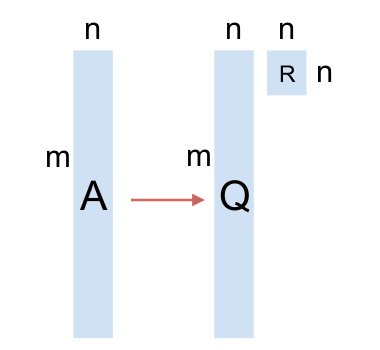
\includegraphics[height=4cm]{qr.png}

Q hesabı için biraz daha takla atmak lazım,

$$A = QR$$

$$AR^{-1} = QRR^{-1} $$

$$Q = AR^{-1} $$

Demek ki $R$'i elde ettikten sonra onu tersine çevirip (inverse) $A$ ile
çarparsak, bu bize $Q$'yu verecek. Dert değil, $R$ ufak bir matris, $n \times
n$, ve tersini alma operasyonu pahalı bir işlem olsa da bu boyutlarda yavaş
olmaz. Daha sonra bu $R^{-1}$'i alıp bu sefer başka bir eşle/indirge ile çarpım
işlemine tabi tutarız. R'yi direk alttaki script içine yazdık (B olarak) bir
sonuç ortamında bu verinin başka bir şekilde MRJob işlemine verilmiş olması
lazım. Bir işleme zinciri var, zincirde önce $A^TA$, Cholesky, oradan $R$ alınıp
başka bir işleme (job) aktarılıyor.

\inputminted[fontsize=\footnotesize]{python}{AB.py}

\begin{minted}[fontsize=\footnotesize]{python}
!python AB.py A_matrix
\end{minted}

\begin{verbatim}
using configs in /home/burak/.mrjob.conf
creating tmp directory /tmp/AB.burak.20131202.230008.985111
writing to /tmp/AB.burak.20131202.230008.985111/step-0-mapper_part-00000
Counters from step 1:
  (no counters found)
writing to /tmp/AB.burak.20131202.230008.985111/step-0-mapper-sorted
> sort /tmp/AB.burak.20131202.230008.985111/step-0-mapper_part-00000
writing to /tmp/AB.burak.20131202.230008.985111/step-0-reducer_part-00000
Counters from step 1:
  (no counters found)
Moving /tmp/AB.burak.20131202.230008.985111/step-0-reducer_part-00000 -> /tmp/AB.burak.20131202.230008.985111/output/part-00000
Streaming final output from /tmp/AB.burak.20131202.230008.985111/output
null	"[[ -61.48170459  -88.78963451  -62.09685608  -84.98432736]\n [ -20.49390153  -27.8454303   -19.85529535  -27.30069639]\n [ -40.98780306  -55.6908606   -39.7105907   -54.60139278]\n [-184.44511377 -250.6088727  -205.35232431 -234.71714361]]"
null	"[[ -61.48170459  -99.29632173  -76.04368486 -131.21677204]\n [ -40.98780306  -55.6908606   -39.7105907   -54.60139278]\n [-184.44511377 -250.6088727  -205.35232431 -234.71714361]\n [ -61.48170459  -88.78963451  -62.09685608 -102.4767312 ]]"
null	"[[-184.44511377 -250.6088727  -205.35232431 -234.71714361]\n [ -61.48170459  -99.29632173  -76.04368486 -131.21677204]\n [ -40.98780306  -55.6908606   -39.7105907   -54.60139278]\n [-184.44511377 -250.6088727  -205.35232431 -234.71714361]]"
null	"[[ -61.48170459  -88.78963451  -62.09685608 -102.4767312 ]\n [ -61.48170459  -88.78963451  -62.09685608  -84.98432736]\n [ -61.48170459  -99.29632173  -76.04368486 -131.21677204]\n [ -40.98780306  -55.6908606   -39.7105907   -54.60139278]]"
removing tmp directory /tmp/AB.burak.20131202.230008.985111
\end{verbatim}

Kontrol edelim,

\begin{minted}[fontsize=\footnotesize]{python}
B = np.array([[-20.49390153,   0.        ,   0.        ,   0.        ],
              [-22.59208669,  -5.25334361,   0.        ,   0.        ],
              [-12.88188096, -11.41585875,   4.44244436,   0.        ],
              [-12.93067597, -12.53849977,   2.54158031,  -4.37310096]])
print np.dot(A,B.T)
\end{minted}

\begin{verbatim}
[[ -61.48170459  -88.78963451  -62.09685608 -102.4767312 ]
 [ -61.48170459  -88.78963451  -62.09685608  -84.98432736]
 [ -61.48170459  -99.29632173  -76.04368486 -131.21677204]
 [ -40.98780306  -55.6908606   -39.7105907   -54.60139278]
 [-184.44511377 -250.6088727  -205.35232431 -234.71714361]
 [ -61.48170459  -99.29632173  -76.04368486 -131.21677204]
 [ -40.98780306  -55.6908606   -39.7105907   -54.60139278]
 [-184.44511377 -250.6088727  -205.35232431 -234.71714361]
 [ -61.48170459  -99.29632173  -76.04368486 -131.21677204]
 [ -40.98780306  -55.6908606   -39.7105907   -54.60139278]
 [-184.44511377 -250.6088727  -205.35232431 -234.71714361]
 [ -61.48170459  -88.78963451  -62.09685608 -102.4767312 ]
 [ -61.48170459  -88.78963451  -62.09685608  -84.98432736]
 [ -20.49390153  -27.8454303   -19.85529535  -27.30069639]
 [ -40.98780306  -55.6908606   -39.7105907   -54.60139278]
 [-184.44511377 -250.6088727  -205.35232431 -234.71714361]
 [ -81.97560612 -116.63506481  -90.83704015 -126.11438629]]
\end{verbatim}

Çarpımlar aynı. Yanlız dikkat, satırların sırası değişik olabilir, burada
problem eşle/indirge işleminin $A$'yi parçalama sonucu her çarpım parçasının
değişik bir sırada ele geçiyor olması. Eğer sıralamayı aynı $A$ gibi istiyorsak,
bu sıra no'sunu $A$ verisi içinde ilk satıra koymak lazım ve eşleyiciler oradan
alıp bu no'yu anahtar olarak yayınlamalılar. Bu eklemeyi okuyucuya bırakıyorum!

Şimdi QR hesabını bu şekilde yapıp yapamayacağımızı kontrol edelim. Eğer
\verb!qr! ile $Q$ hesaplarsak,

\begin{minted}[fontsize=\footnotesize]{python}
q,r = lin.qr(A)
print q
\end{minted}

\begin{verbatim}
[[-0.14638501 -0.13188879  0.36211188 -0.35057934]
 [-0.14638501 -0.13188879  0.36211188  0.56410341]
 [-0.14638501 -0.51259871 -0.16600517 -0.02328772]
 [-0.09759001  0.03897744  0.26737941 -0.1251395 ]
 [-0.43915503  0.1753985  -0.14740047  0.02394349]
 [-0.14638501 -0.51259871 -0.16600517 -0.02328772]
 [-0.09759001  0.03897744  0.26737941 -0.1251395 ]
 [-0.43915503  0.1753985  -0.14740047  0.02394349]
 [-0.14638501 -0.51259871 -0.16600517 -0.02328772]
 [-0.09759001  0.03897744  0.26737941 -0.1251395 ]
 [-0.43915503  0.1753985  -0.14740047  0.02394349]
 [-0.14638501 -0.13188879  0.36211188 -0.35057934]
 [-0.14638501 -0.13188879  0.36211188  0.56410341]
 [-0.048795    0.01948872  0.1336897  -0.06256975]
 [-0.09759001  0.03897744  0.26737941 -0.1251395 ]
 [-0.43915503  0.1753985  -0.14740047  0.02394349]
 [-0.19518001 -0.11240007  0.04559899 -0.21745867]]
\end{verbatim}

$R$'in tersi ile $A$ carpilinca hakikaten $Q$ elde ediliyor mu?
Kontrol edelim.

\begin{minted}[fontsize=\footnotesize]{python}
print np.dot(A,lin.inv(B.T))
\end{minted}

\begin{verbatim}
[[-0.14638501 -0.13188879  0.36211188 -0.35057934]
 [-0.14638501 -0.13188879  0.36211188  0.56410341]
 [-0.14638501 -0.51259871 -0.16600517 -0.02328772]
 [-0.09759001  0.03897744  0.26737941 -0.1251395 ]
 [-0.43915503  0.1753985  -0.14740047  0.02394349]
 [-0.14638501 -0.51259871 -0.16600517 -0.02328772]
 [-0.09759001  0.03897744  0.26737941 -0.1251395 ]
 [-0.43915503  0.1753985  -0.14740047  0.02394349]
 [-0.14638501 -0.51259871 -0.16600517 -0.02328772]
 [-0.09759001  0.03897744  0.26737941 -0.1251395 ]
 [-0.43915503  0.1753985  -0.14740047  0.02394349]
 [-0.14638501 -0.13188879  0.36211188 -0.35057934]
 [-0.14638501 -0.13188879  0.36211188  0.56410341]
 [-0.048795    0.01948872  0.1336897  -0.06256975]
 [-0.09759001  0.03897744  0.26737941 -0.1251395 ]
 [-0.43915503  0.1753985  -0.14740047  0.02394349]
 [-0.19518001 -0.11240007  0.04559899 -0.21745867]]
\end{verbatim}

Sonuçlar birebir aynı.

Üstteki teknikleri kullanarak artık devasa boyutlarda satırı olan bir $A$
matrisi üzerinde artık QR hesabı yapılabilir.

SVD

Peki $QR$ sonuçlarını kullanarak SVD sonuçlarını alabilir miyiz?  SVD bize ne
verir?

$$ A = U \Sigma V^T $$

$U$ ve $V^T$ dikgen (orthogonal) matrislerdir, $\Sigma$ sadece köşegeni
boyunca değerleri olan bir matristir. Daha fazla detay için bkz [4]. Şimdi
$A = QR$ yerine koyalım,

$$ QR =  U \Sigma V^T $$

$$ R = Q^T U \Sigma V^T $$

Bu son formüledeki $Q^TU$ ibaresi, iki dikgen matrisin çarpımıdır. Lineer Cebir
kurallarına göre iki dikgen matrisin çarpımı bir diğer ortogonal matristir. Bu
yeni dikgen matrise $U_R$ adı verelim, o zaman

$$ R = U_R \Sigma V^T $$

Bu son formül bize bir şeyler söylüyor. $R$'nin SVD üzerinden
ayrıştırılabileceğini söylüyor ve bu ayrıştırma sonrası ele geçen $U_R,V^T$ ve
$\Sigma$ köşegen matrisleridir! Bu çok önemli bir sonuç.  Bu ayrıştırmanın
sonucu $A$'nin ki ile birbirine çok benziyor, tek fark $U$ ile $U_R$. Bu iki
matris arasındaki geçiş şöyle:

$$ U_R = Q^T U $$ 

$$ U = QU_R $$ 

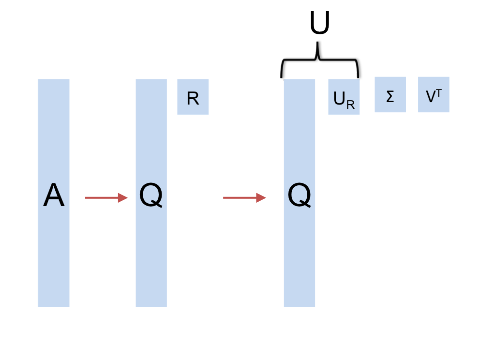
\includegraphics[height=6cm]{ur.png}

Bu demektir ki eğer $R$ üzerinde kütüphanemizin \verb!svd!  çağrısını
kullanırsak (ki $R$ nispeten ufak olduğu için bu ucuz olur) ele geçen $U_R$'i
alıp, $Q$ ile çarparsak, $A$ ayrıştırmasının $U$'şunu elde ederiz! $Q$ ile
çarpım eşle/indirge üzerinden yapılabilir, fakat basit bir çarpım işlemi olduğu
için paralelize edilmesi kolaydır (üstteki mrjob script'inde yaptığımız gibi).

Kaynaklar

[1] Benson, A., {\em Tall-and-skinny Matrix Computations in MapReduce}

[2] Constantine, P. G., Gleich, D. F. , {\em Tall and Skinny QR factorizations in MapReduce architectures}

[3] Dasgupta, S., Gupta, A., {\em An Elementary Proof of a Theorem of Johnson and Lindenstrauss}

[4] Bayramli, Lineer Cebir, {\em Ders 29}

[5] Bayramli, Lineer Cebir, {\em Matris Çarpımı, Ders 1}


\end{document}
